\documentclass[12pt,letterpaper]{report}
\usepackage[utf8]{inputenc}
\usepackage{amsmath}
\usepackage{amsfonts}
\usepackage{amssymb}
\usepackage{pdfpages}
\usepackage[left=0.50in, right=0.50in, bottom=0.50in, top=0.50in]{geometry}
\author{National Conference of Volunteer Examiners; edited by Anthony Odenthal KE7OSN}
\title{Amateur Radio Technician Class Exam Questions and Answers for July 2010 to July 2014}
\begin{document}
\maketitle
\section{Preamble}

The following is the entire question pool for the Technician class amateur radio exam with answers. The text comes from the NCVEC National Conference of Volunteer Examiners website http://www.ncvec.org/page.php?id=349 on November 21 2013 and edited to remove the distractors (wrong answers). For questions with the answer "All of the above" the distractors were left in place for the information of anyone using this document. This document also lacks the list of corrections and modifications the original had.

Each subelement indicates the number of groups and the number of exam questions that comes form that subelement. Questions are formatted as Question Number (Letter of the correct Answer) [FCC rule number if applicable] question, the letter and answer for the correct response is listed on the second line.

\tableofcontents
\chapter*{Syllabus}
SUBELEMENT T1   FCC Rules, descriptions and definitions for the amateur radio service, operator and station license responsibilities - [6 Exam Questions - 6 Groups]\\

T1A - Amateur Radio services; purpose of the amateur service, amateur-satellite service, operator/primary station license grant, where FCC rules are codified, basis and purpose of FCC rules, meanings of basic terms used in FCC rules

T1B - Authorized frequencies; frequency allocations, ITU regions, emission type, restricted sub-bands, spectrum sharing, transmissions near band edges

T1C - Operator classes and station call signs; operator classes, sequential, special event, and vanity call sign systems, international communications, reciprocal operation, station license licensee, places where the amateur service is regulated by the FCC, name and address on ULS, license term, renewal, grace period

T1D - Authorized and prohibited transmissions

T1E - Control operator and control types; control operator required, eligibility, designation of control operator, privileges and duties, control point, local, automatic and remote control, location of control operator 

T1F - Station identification and operation standards; special operations for repeaters and auxiliary stations, third party communications, club stations, station security, FCC inspection\\


SUBELEMENT T2 - Operating Procedures - [3 Exam Questions - 3 Groups]\\

T2A - Station operation; choosing an operating frequency, calling another station, test transmissions, use of minimum power, frequency use, band plans

T2B   VHF/UHF operating practices; SSB phone, FM repeater, simplex, frequency offsets, splits and shifts, CTCSS, DTMF, tone squelch, carrier squelch, phonetics

T2C  Public service; emergency and non-emergency operations, message traffic handling\\


SUBELEMENT T3   Radio wave characteristics, radio and electromagnetic properties, propagation modes   [3 Exam Questions - 3 Groups]\\

T3A - Radio wave characteristics; how a radio signal travels; distinctions of HF, VHF and UHF; fading, multipath; wavelength vs. penetration; antenna orientation

T3B - Radio and electromagnetic wave properties; the electromagnetic spectrum, wavelength vs. frequency, velocity of electromagnetic waves 

T3C - Propagation modes; line of sight, sporadic E, meteor, aurora scatter, tropospheric ducting, F layer skip, radio horizon\\


SUBELEMENT T4 - Amateur radio practices and station setup   [2 Exam Questions - 2 Groups]\\

T4A   Station setup; microphone, speaker, headphones, filters, power source, connecting a computer, RF grounding

T4B - Operating controls; tuning, use of filters, squelch, AGC, repeater offset, memory channels\\


SUBELEMENT T5   Electrical principles, math for electronics, electronic principles, Ohm s Law   [4 Exam Questions - 4 Groups]\\

T5A - Electrical principles; current and voltage, conductors and insulators, alternating and direct current

T5B - Math for electronics; decibels, electronic units and the metric system

T5C - Electronic principles; capacitance, inductance, current flow in circuits, alternating current, definition of RF, power calculations

T5D   Ohm s Law\\


SUBELEMENT T6   Electrical components, semiconductors, circuit diagrams, component functions   [4 Exam Groups - 4 Questions]\\

T6A - Electrical components; fixed and variable resistors, capacitors, and inductors; fuses, switches, batteries

T6B   Semiconductors; basic principles of diodes and transistors

T6C - Circuit diagrams; schematic symbols

T6D - Component functions\\


SUBELEMENT T7   Station equipment, common transmitter and receiver problems, antenna measurements and troubleshooting, basic repair and testing   [4 Exam Questions - 4 Groups]\\

T7A - Station radios; receivers, transmitters, transceivers

T7B   Common transmitter and receiver problems; symptoms of overload and overdrive, distortion, interference, over and under modulation, RF feedback, off frequency signals; fading and noise; problems with digital communications interfaces

T7C   Antenna measurements and troubleshooting; measuring SWR, dummy loads, feedline failure modes

T7D   Basic repair and testing; soldering, use of a voltmeter, ammeter, and ohmmeter\\



SUBELEMENT T8   Modulation modes, amateur satellite operation, operating activities, non-voice communications   [4 Exam Questions - 4 Groups]\\

T8A   Modulation modes; bandwidth of various signals

T8B - Amateur satellite operation; Doppler shift, basic orbits, operating protocols

T8C   Operating activities; radio direction finding, radio control, contests, special event stations, basic linking over Internet

T8D   Non-voice communications; image data, digital modes, CW, packet, PSK31\\


SUBELEMENT T9   Antennas, feedlines [2 Exam Groups - 2 Questions]\\

T9A   Antennas; vertical and horizontal, concept of gain, common portable and mobile antennas, relationships between antenna length and frequency

T9B - Feedlines; types, losses vs. frequency, SWR concepts, matching, weather protection, connectors\\


SUBELEMENT T0   AC power circuits, antenna installation, RF hazards   [3 Exam Questions - 3 Groups]\\

T0A   AC power circuits; hazardous voltages, fuses and circuit breakers, grounding, lightning protection, battery safety, electrical code compliance

T0B   Antenna installation; tower safety, overhead power lines

T0C - RF hazards; radiation exposure, proximity to antennas, recognized safe power levels, exposure to others


\chapter{Subelement T1 - FCC Rules, descriptions and definitions for the amateur radio service, operator and station license responsibilities: 6 Questions}
\section{T1A - Amateur Radio services; purpose of the amateur service, amateur-satellite service, operator/primary station license grant, where FCC rules are codified, basis and purpose of FCC rules, meanings of basic terms used in FCC rules}

T1A01 (D) [97.3(a)(4)] For whom is the Amateur Radio Service intended?\\
D. Persons who are interested in radio technique solely with a personal aim and without pecuniary interest\\

T1A02 (C) [97.1] What agency regulates and enforces the rules for the Amateur Radio Service in the United States?\\
C. The FCC\\

T1A03 (D) Which part of the FCC rules contains the rules and regulations governing the Amateur Radio Service?\\
D. Part 97\\

T1A04 (C) [97.3(a)(23)] Which of the following meets the FCC definition of harmful interference?\\
C. That which seriously degrades, obstructs, or repeatedly interrupts a radio communication service operating in accordance with the Radio Regulations\\

T1A05 (D) [97.3(a)(40)] What is the FCC Part 97 definition of a space station?\\
D. An amateur station located more than 50 km above the Earth's surface\\

T1A06 (C) [97.3(a)(43)] What is the FCC Part 97 definition of telecommand?\\
C. A one-way transmission to initiate, modify or terminate functions of a device at a distance\\

T1A07 (C) [97.3(a)(45)] What is the FCC Part 97 definition of telemetry?\\
C. A one-way transmission of measurements at a distance from the measuring instrument D. An information bulletin from a VEC\\

T1A08 (B) [97.3(a)(22)] Which of the following entities recommends transmit/receive channels and other parameters for auxiliary and repeater stations?\\
B. Frequency Coordinator\\

T1A09 (C) [97.3(a)(22)] Who selects a Frequency Coordinator?\\
C. Amateur operators in a local or regional area whose stations are eligible to be auxiliary or repeater stations\\

T1A10 (A) [97.3(a)(5)] What is the FCC Part 97 definition of an amateur station?\\
A. A station in an Amateur Radio Service consisting of the apparatus necessary for carrying on radio communications\\

T1A11 (C) [97.3(a)(7)] Which of the following stations transmits signals over the air from a remote receive site to a repeater for retransmission?\\
C. Auxiliary station\\

\section{T1B - Authorized frequencies; frequency allocations, ITU regions, emission type, restricted sub-bands, spectrum sharing, transmissions near band edges}

T1B01 (B) [97.3(a)(28)] What is the ITU?\\
B. A United Nations agency for information and communication technology issues\\

T1B02 (B) North American amateur stations are located in which ITU region?\\
B. Region 2\\

T1B03 (B) [97.301(a)] Which frequency is within the 6 meter band?\\
B. 52.525 MHz\\

T1B04 (A) [97.301(a)] Which amateur band are you using when your station is transmitting on 146.52 MHz?\\
A. 2 meter band\\

T1B05 (C) [97.301(a)] Which 70 cm frequency is authorized to a Technician Class license holder operating in ITU Region 2?\\
C. 443.350 MHz\\

T1B06 (B) [97.301(a)] Which 23 cm frequency is authorized to a Technician Class operator license?\\
B. 1296 MHz\\

T1B07 (D) [97.301(a)] What amateur band are you using if you are transmitting on 223.50 MHz?\\
D. 1.25 meter band\\

T1B08 (C) [97.303] What do the FCC rules mean when an amateur frequency band is said to be available on a secondary basis?\\
C. Amateurs may not cause harmful interference to primary users\\

T1B09 (D) [97.101(a)] Why should you not set your transmit frequency to be exactly at the edge of an amateur band or sub-band?\\
A. To allow for calibration error in the transmitter frequency display\\
B. So that modulation sidebands do not extend beyond the band edge\\
C. To allow for transmitter frequency drift\\
D. All of these choices are correct\\

T1B10 (C) [97.305(c)] Which of the bands available to Technician Class operators have mode-restricted sub-bands?\\
C. The 6 meter, 2 meter, and 1.25 meter bands\\

T1B11 (A) [97.305 (a)(c)] What emission modes are permitted in the mode-restricted sub-bands at 50.0 to 50.1 MHz and 144.0 to 144.1 MHz?\\
A. CW only\\

\section{T1C - Operator classes and station call signs; operator classes, sequential, special event, and vanity call sign systems, international communications, reciprocal operation, station license and licensee, places where the amateur service is regulated by the FCC, name and address on ULS, license term, renewal, grace period}

T1C01 (C) [97.3(a)(11)(iii)] Which type of call sign has a single letter in both the prefix and suffix?\\
C. Special event\\

T1C02 (B) Which of the following is a valid US amateur radio station call sign?\\
B. W3ABC\\

T1C03 (A) [97.117] What types of international communications are permitted by an FCC-licensed amateur station?\\
A. Communications incidental to the purposes of the amateur service and remarks of a personal character\\

T1C04 (A) When are you allowed to operate your amateur station in a foreign country?\\
A. When the foreign country authorizes it\\

T1C05 (A) [97.303(h)] What must you do if you are operating on the 23 cm band and learn that you are interfering with a radiolocation station outside the United States?\\
A. Stop operating or take steps to eliminate the harmful interference\\

T1C06 (D) [97.5(a)(2)] From which of the following may an FCC-licensed amateur station transmit, in addition to places where the FCC regulates communications?\\
D. From any vessel or craft located in international waters and documented or registered in the United States\\

T1C07 (B) [97.23] What may result when correspondence from the FCC is returned as undeliverable because the grantee failed to provide the correct mailing address?\\
B. Revocation of the station license or suspension of the operator license\\

T1C08 (C) [97.25] What is the normal term for an FCC-issued primary station/operator license grant?\\
C. Ten years\\

T1C09 (A) [97.21(a)(b)] What is the grace period following the expiration of an amateur license within which the license may be renewed?\\
A. Two years\\

T1C10 (C) [97.5a] How soon may you operate a transmitter on an amateur service frequency after you pass the examination required for your first amateur radio license?\\
C. As soon as your name and call sign appear in the FCC s ULS database\\

T1C11 (A) [97.21(b)] If your license has expired and is still within the allowable grace period, may you continue to operate a transmitter on amateur service frequencies?\\
A. No, transmitting is not allowed until the ULS database shows that the license has been renewed\\

\section{T1D - Authorized and prohibited transmissions}

T1D01 (A) [97.111(a)(1)] With which countries are FCC-licensed amateur stations prohibited from exchanging communications?\\
A. Any country whose administration has notified the ITU that it objects to such communications\\

T1D02 (A) [97.111(a)(5)] On which of the following occasions may an FCC-licensed amateur station exchange messages with a U.S. military station?\\
A. During an Armed Forces Day Communications Test\\

T1D03 (C) [97.113(a)(4), 97.211(b), 97.217] When is the transmission of codes or ciphers allowed to hide the meaning of a message transmitted by an amateur station?\\
C. Only when transmitting control commands to space stations or radio control craft\\

T1D04 (A) [97.113(a)(4), 97.113(e)] What is the only time an amateur station is authorized to transmit music?\\
A. When incidental to an authorized retransmission of manned spacecraft communications\\

T1D05 (A) [97.113(a)(3)] When may amateur radio operators use their stations to notify other amateurs of the availability of equipment for sale or trade?\\
A. When the equipment is normally used in an amateur station and such activity is not conducted on a regular basis\\

T1D06 (A) [97.113(a)(4)] Which of the following types of transmissions are prohibited?\\
A. Transmissions that contain obscene or indecent words or language\\

T1D08 (B) [97.113] When may the control operator of an amateur station receive compensation for operating the station? \\
B. When the communication is incidental to classroom instruction at an educational institution\\

T1D09 (A) [97.113(b)] Under which of the following circumstances are amateur stations authorized to transmit signals related to broadcasting, program production, or news gathering, assuming no other means is available?\\
A. Only where such communications directly relate to the immediate safety of human life or protection of property\\

T1D10 (D) [97.3(a)(10)] What is the meaning of the term broadcasting in the FCC rules for the amateur services?\\
D. Transmissions intended for reception by the general public \\

T1D11 (A) [97.113(a)(5)] Which of the following types of communications are permitted in the Amateur Radio Service?\\
A. Brief transmissions to make station adjustments\\

\section{T1E - Control operator and control types; control operator required, eligibility, designation of control operator, privileges and duties, control point, local, automatic and remote control, location of control operator}

T1E01 (A) [97.7(a)] When must an amateur station have a control operator?\\
A. Only when the station is transmitting\\

T1E02 (D) [97.7(a)] Who is eligible to be the control operator of an amateur station?\\
D. Only a person for whom an amateur operator/primary station license grant appears in the FCC database or who is authorized for alien reciprocal operation\\

T1E03 (A) [97.103(b)] Who must designate the station control operator?\\
A. The station licensee\\

T1E04 (D) [97.103(b)] What determines the transmitting privileges of an amateur station?\\
D. The class of operator license held by the control operator\\

T1E05 (C) [97.3(a)(14)] What is an amateur station control point?
C. The location at which the control operator function is performed

T1E06 (B) [97.109(d)] Under which of the following types of control is it permissible for the control operator to be at a location other than the control point?\\
B. Automatic control\\

T1E07 (D) [97.103(a)] When the control operator is not the station licensee, who is responsible for the proper operation of the station?\\
D. The control operator and the station licensee are equally responsible\\

T1E08 (C) [97.3(a)] What type of control is being used for a repeater when the control operator is not present at a control point?\\
C. Automatic control\\

T1E09 (D) [97.109(a)] What type of control is being used when transmitting using a handheld radio?\\
D. Local control\\

T1E10 (B) [97.3] What type of control is used when the control operator is not at the station location but can indirectly manipulate the operating adjustments of a station?\\
B. Remote\\

T1E11 (D) [97.103(a)] Who does the FCC presume to be the control operator of an amateur station, unless documentation to the contrary is in the station records?\\
D. The station licensee\\

\section{T1F - Station identification and operation standards; special operations for repeaters and auxiliary stations, third party communications, club stations, station security, FCC inspection}

T1F01 (A) What type of identification is being used when identifying a station on the air as  Race Headquarters ?\\
A. Tactical call\\

T1F02 (C) [97.119 (a)] When using tactical identifiers, how often must your station transmit the station s FCC-assigned call sign? \\
C. Every ten minutes\\

T1F03 (D) [97.119(a)] When is an amateur station required to transmit its assigned call sign?\\
D. At least every 10 minutes during and at the end of a contact\\

T1F04 (C) [97.119(b)] Which of the following is an acceptable language for use for station identification when operating in a phone sub-band?\\
C. The English language\\

T1F05 (B) [97.119(b)] What method of call sign identification is required for a station transmitting phone signals?\\
B. Send the call sign using CW or phone emission\\

T1F06 (D) [97.119(c)] Which of the following formats of a self-assigned indicator is acceptable when identifying using a phone transmission?\\
A. KL7CC stroke W3\\
B. KL7CC slant W3\\
C. KL7CC slash W3\\
D. All of these choices are correct\\

T1F07 (D) [97.119(c)] Which of the following restrictions apply when appending a self-assigned call sign indicator?\\
D. It must not conflict with any other indicator specified by the FCC rules or with any call sign prefix assigned to another country\\

T1F08 (A) [97.119(e)] When may a Technician Class licensee be the control operator of a station operating in an exclusive Extra Class operator segment of the amateur bands?\\
A. Never\\

T1F09 (C) [97.3(a)(39)] What type of amateur station simultaneously retransmits the signal of another amateur station on a different channel or channels?\\
C. Repeater station\\

T1F10 (A) [97.205(g)] Who is accountable should a repeater inadvertently retransmit communications that violate the FCC rules?\\
A. The control operator of the originating station\\

T1F11 (A) [97.115(a)] To which foreign stations do the FCC rules authorize the transmission of non-emergency third party communications?\\
A. Any station whose government permits such communications\\

T1F12 (B) [97.5(b)(2)] How many persons are required to be members of a club for a club station license to be issued by the FCC?\\
B. At least 4\\

T1F13 (B) [97.103(c)] When must the station licensee make the station and its records available for FCC inspection? \\
B. Any time upon request by an FCC representative\\

\chapter{Subelement T2 - Operating Procedures: 3 Questions}
\section{T2A - Station operation; choosing an operating frequency, calling another station, test transmissions, use of minimum power, frequency use, band plans}

T2A01 (B) What is the most common repeater frequency offset in the 2 meter band?\\
B. plus or minus 600 kHz\\

T2A02 (D) What is the national calling frequency for FM simplex operations in the 70 cm band?\\
D. 446.000 MHz\\

T2A03 (A) What is a common repeater frequency offset in the 70 cm band?\\
A. Plus or minus 5 MHz\\

T2A04 (B) What is an appropriate way to call another station on a repeater if you know the other station's call sign?\\
B. Say the station's call sign then identify with your call sign\\

T2A05 (C) What should you transmit when responding to a call of CQ?\\
C. The other station's call sign followed by your call sign\\

T2A06 (A) What must an amateur operator do when making on-air transmissions to test equipment or antennas?\\
A. Properly identify the transmitting station\\

T2A07 (D) Which of the following is true when making a test transmission?\\
D. Station identification is required at least every ten minutes during the test and at the end\\

T2A08 (D) What is the meaning of the procedural signal "CQ"?\\
D. Calling any station\\

T2A09 (B) What brief statement is often used in place of "CQ" to indicate that you are listening on a repeater?\\
B. Say your call sign  \\

T2A10 (A) What is a band plan, beyond the privileges established by the FCC?\\
A. A voluntary guideline for using different modes or activities within an amateur band\\

T2A11 (D) [97.313(a)] What are the FCC rules regarding power levels used in the amateur bands?\\
D. An amateur must use the minimum transmitter power necessary to carry out the desired communication\\

\section{T2B - VHF/UHF operating practices; SSB phone, FM repeater, simplex, frequency offsets, splits and shifts, CTCSS, DTMF, tone squelch, carrier squelch, phonetics}

T2B01 (C) What is the term used to describe an amateur station that is transmitting and receiving on the same frequency?\\
C. Simplex communication\\

T2B02 (D) What is the term used to describe the use of a sub-audible tone transmitted with normal voice audio to open the squelch of a receiver?\\
D. CTCSS\\

T2B03 (B) Which of the following describes the muting of receiver audio controlled solely by the presence or absence of an RF signal?\\
B. Carrier squelch\\

T2B04 (D) Which of the following common problems might cause you to be able to hear but not access a repeater even when transmitting with the proper offset?\\
A. The repeater receiver requires audio tone burst for access\\
B. The repeater receiver requires a CTCSS tone for access\\
C. The repeater receiver may require a DCS tone sequence for access\\
D. All of these choices are correct\\

T2B05 (C) What determines the amount of deviation of an FM signal?\\
C. The amplitude of the modulating signal\\

T2B06 (A) What happens when the deviation of an FM transmitter is increased?\\
A. Its signal occupies more bandwidth\\

T2B07 (D) What should you do if you receive a report that your station s transmissions are causing splatter or interference on nearby frequencies?\\
D. Check your transmitter for off-frequency operation or spurious emissions\\

T2B08 (B) What is the proper course of action if your station s transmission unintentionally interferes with another station?\\
B. Properly identify your transmission and move to a different frequency\\

T2B09 (A) [97.119(b)(2)] Which of the following methods is encouraged by the FCC when identifying your station when using phone?\\
A. Use of a phonetic alphabet\\

T2B10 (A) What is the "Q" signal used to indicate that you are receiving interference from other stations?\\
A. QRM\\

T2B11 (B) What is the "Q" signal used to indicate that you are changing frequency?\\
B. QSY\\

\section{T2C - Public service; emergency and non-emergency operations, message traffic handling}

T2C01 (C) [97.103(a)] What set of rules applies to proper operation of your station when using amateur radio at the request of public service officials?\\
C. FCC Rules\\

T2C04 (D) What do RACES and ARES have in common?\\
D. Both organizations may provide communications during emergencies\\

T2C05 (B) [97.3(a)(37), 97.407 ] What is the Radio Amateur Civil Emergency Service?\\
B. A radio service using amateur stations for emergency management or civil defense communications\\

T2C06 (C) Which of the following is common practice during net operations to get the immediate attention of the net control station when reporting an emergency?\\
C. Begin your transmission with  Priority  or  Emergency  followed by your call sign\\

T2C07 (C) What should you do to minimize disruptions to an emergency traffic net once you have checked in?\\
C. Do not transmit on the net frequency until asked to do so by the net control station\\

T2C08 (A) What is usually considered to be the most important job of an amateur operator when handling emergency traffic messages?\\
A. Passing messages exactly as written, spoken or as received\\

T2C09 (B) [97.403] When may an amateur station use any means of radio communications at its disposal for essential communications in connection with immediate safety of human life and protection of property?\\
B. When normal communications systems are not available\\

T2C10 (D) What is the preamble in a formal traffic message?\\
D. The information needed to track the message as it passes through the amateur radio traffic handling system\\

T2C11 (A) What is meant by the term "check" in reference to a formal traffic message?\\
A. The check is a count of the number of words or word equivalents in the text portion of the message\\

\chapter{Subelement T3 - Radio wave characteristics, radio and electromagnetic properties, propagation modes: 3 Questions}

\section{T3A - Radio wave characteristics; how a radio signal travels; distinctions of HF, VHF and UHF; fading, multipath; wavelength vs. penetration; antenna orientation}

T3A01 (D) What should you do if another operator reports that your station s 2 meter signals were strong just a moment ago, but now they are weak or distorted?\\
D. Try moving a few feet, as random reflections may be causing multi-path distortion\\

T3A02 (B) Why are UHF signals often more effective from inside buildings than VHF signals?\\
B. The shorter wavelength allows them to more easily penetrate the structure of buildings\\

T3A03 (C) What antenna polarization is normally used for long-distance weak-signal CW and SSB contacts using the VHF and UHF bands?\\
C. Horizontal\\

T3A04 (B) What can happen if the antennas at opposite ends of a VHF or UHF line of sight radio link are not using the same polarization?\\
B. Signals could be significantly weaker\\

T3A05 (B) When using a directional antenna, how might your station be able to access a distant repeater if buildings or obstructions are blocking the direct line of sight path?\\
B. Try to find a path that reflects signals to the repeater\\

T3A06 (B) What term is commonly used to describe the rapid fluttering sound sometimes heard from mobile stations that are moving while transmitting?\\
B. Picket fencing\\

T3A07 (A) What type of wave carries radio signals between transmitting and receiving stations?
A. Electromagnetic

T3A08 (C) What is the cause of irregular fading of signals from distant stations during times of generally good reception?\\
C. Random combining of signals arriving via different path lengths\\

T3A09 (B) Which of the following is a common effect of "skip" reflections between the Earth and the ionosphere?\\
B. The polarization of the original signal is randomized\\

T3A10 (D) What may occur if VHF or UHF data signals propagate over multiple paths?\\
D. Error rates are likely to increase\\

T3A11 (C) Which part of the atmosphere enables the propagation of radio signals around the world?\\
C. The ionosphere\\

\section{T3B - Radio and electromagnetic wave properties; the electromagnetic spectrum, wavelength vs. frequency, velocity of electromagnetic waves}

T3B01 (C) What is the name for the distance a radio wave travels during one complete cycle?\\
C. Wavelength\\

T3B02 (D) What term describes the number of times per second that an alternating current reverses direction?\\
D. Frequency\\

T3B03 (C) What are the two components of a radio wave?\\
C. Electric and magnetic fields\\

T3B04 (A) How fast does a radio wave travel through free space?\\
A. At the speed of light\\

T3B05 (B) How does the wavelength of a radio wave relate to its frequency?\\
B. The wavelength gets shorter as the frequency increases\\

T3B06 (D) What is the formula for converting frequency to wavelength in meters?\\
D. Wavelength in meters equals 300 divided by frequency in megahertz\\

T3B07 (A) What property of radio waves is often used to identify the different frequency bands?\\
A. The approximate wavelength\\

T3B08 (B) What are the frequency limits of the VHF spectrum?\\
B. 30 to 300 MHz\\

T3B09 (D) What are the frequency limits of the UHF spectrum?\\
D. 300 to 3000 MHz\\

T3B10 (C) What frequency range is referred to as HF?\\
C. 3 to 30 MHz\\

T3B11 (B) What is the approximate velocity of a radio wave as it travels through free space?\\
B. 300,000,000 meters per second\\

\section{T3C - Propagation modes; line of sight, sporadic E, meteor, aurora scatter, tropospheric ducting, F layer skip, radio horizon}

T3C01 (C) Why are "direct" (not via a repeater) UHF signals rarely heard from stations outside your local coverage area?\\
C. UHF signals are usually not reflected by the ionosphere\\

T3C02 (D) Which of the following might be happening when VHF signals are being received from long distances?\\
D. Signals are being refracted from a sporadic E layer\\

T3C03 (B) What is a characteristic of VHF signals received via auroral reflection?\\
B. The signals exhibit rapid fluctuations of strength and often sound distorted\\

T3C04 (B) Which of the following propagation types is most commonly associated with occasional strong over-the-horizon signals on the 10, 6, and 2 meter bands?\\
B. Sporadic E\\

T3C05 (C) What is meant by the term "knife-edge" propagation?\\
C. Signals are partially refracted around solid objects exhibiting sharp edges\\

T3C06 (A) What mode is responsible for allowing over-the-horizon VHF and UHF communications to ranges of approximately 300 miles on a regular basis?\\
A. Tropospheric scatter\\

T3C07 (B) What band is best suited to communicating via meteor scatter?\\
B. 6 meters\\

T3C08 (D) What causes "tropospheric ducting"?\\
D. Temperature inversions in the atmosphere\\

T3C09 (A) What is generally the best time for long-distance 10 meter band propagation?\\
A. During daylight hours\\

T3C10 (A) What is the radio horizon?\\
A. The distance at which radio signals between two points are effectively blocked by the curvature of the Earth\\

T3C11 (C) Why do VHF and UHF radio signals usually travel somewhat farther than the visual line of sight distance between two stations?\\
C. The Earth seems less curved to radio waves than to light\\

\chapter{Subelement T4 - Amateur radio practices and station set up: 2 Questions}
\section{T4A - Station setup; microphone, speaker, headphones, filters, power source, connecting a computer, RF grounding}

T4A01 (B) Which of the following is true concerning the microphone connectors on amateur transceivers?\\
B. Some connectors include push-to-talk and voltages for powering the microphone\\

T4A02 (C) What could be used in place of a regular speaker to help you copy signals in a noisy area?\\
C. A set of headphones\\

T4A03 (A) Which is a good reason to use a regulated power supply for communications equipment?\\
A. It prevents voltage fluctuations from reaching sensitive circuits\\

T4A04 (A) Where must a filter be installed to reduce harmonic emissions?\\
A. Between the transmitter and the antenna\\

T4A05 (D) What type of filter should be connected to a TV receiver as the first step in trying to prevent RF overload from a nearby 2 meter transmitter?\\
D. Band-reject filter\\

T4A06 (C) Which of the following would be connected between a transceiver and computer in a packet radio station?\\
C. Terminal node controller\\

T4A07 (C) How is the computer s sound card used when conducting digital communications using a computer?\\
C. The sound card provides audio to the microphone input and converts received audio to digital form\\

T4A08 (D) Which type of conductor is best to use for RF grounding?\\
D. Flat strap\\

T4A09 (D) Which would you use to reduce RF current flowing on the shield of an audio cable?\\
D. Ferrite choke\\

T4A10 (B) What is the source of a high-pitched whine that varies with engine speed in a mobile transceiver s receive audio?\\
B. The alternator\\

T4A11 (A) Where should a mobile transceiver's power negative connection be made?\\
A. At the battery or engine block ground strap\\

\section{T4B - Operating controls; tuning, use of filters, squelch, AGC, repeater offset, memory channels}

T4B01 (B) What may happen if a transmitter is operated with the microphone gain set too high?\\
B. The output signal might become distorted\\

T4B02 (A) Which of the following can be used to enter the operating frequency on a modern transceiver?\\
A. The keypad or VFO knob\\

T4B03 (D) What is the purpose of the squelch control on a transceiver?\\
D. To mute receiver output noise when no signal is being received\\

T4B04 (B) What is a way to enable quick access to a favorite frequency on your transceiver?\\
B. Store the frequency in a memory channel\\

T4B05 (C) Which of the following would reduce ignition interference to a receiver?\\
C. Turn on the noise blanker\\

T4B06 (D) Which of the following controls could be used if the voice pitch of a single-sideband signal seems too high or low?\\
D. The receiver RIT or clarifier\\

T4B07 (B) What does the term "RIT" mean?\\
B. Receiver Incremental Tuning\\

T4B08 (B) What is the advantage of having multiple receive bandwidth choices on a multimode transceiver?\\
B. Permits noise or interference reduction by selecting a bandwidth matching the mode\\

T4B09 (C) Which of the following is an appropriate receive filter to select in order to minimize noise and interference for SSB reception?\\
C. 2400 Hz\\

T4B10 (A) Which of the following is an appropriate receive filter to select in order to minimize noise and interference for CW reception?\\
A. 500 Hz\\

T4B11 (C) Which of the following describes the common meaning of the term  repeater offset ?\\
C. The difference between the repeater s transmit and receive frequencies\\

\chapter{Subelemnt T5 - Electrical principles, math for electronics, electronic principles, Ohm s Law: 4 Questions}

\section{T5A - Electrical principles; current and voltage, conductors and insulators, alternating and direct current}

T5A01 (D) Electrical current is measured in which of the following units?\\
D. Amperes\\

T5A02 (B) Electrical power is measured in which of the following units?\\
B. Watts\\

T5A03 (D) What is the name for the flow of electrons in an electric circuit?\\
D. Current \\

T5A04 (B) What is the name for a current that flows only in one direction?\\
B. Direct current\\

T5A05 (A) What is the electrical term for the electromotive force (EMF) that causes electron flow?\\
A. Voltage\\

T5A06 (A) How much voltage does a mobile transceiver usually require?\\
A. About 12 volts\\

T5A07 (C) Which of the following is a good electrical conductor?\\
C. Copper\\

T5A08 (B) Which of the following is a good electrical insulator?\\
B. Glass\\

T5A09 (A) What is the name for a current that reverses direction on a regular basis?\\
A. Alternating current\\

T5A10 (C) Which term describes the rate at which electrical energy is used?\\
C. Power\\

T5A11 (A) What is the basic unit of electromotive force?\\
A. The volt\\

\section{T5B - Math for electronics; decibels, electrical units and the metric system}

T5B01 (C) How many milliamperes is 1.5 amperes?\\
C. 1,500 milliamperes\\

T5B02 (A) What is another way to specify a radio signal frequency of 1,500,000 hertz?\\
A. 1500 kHz\\

T5B03 (C) How many volts are equal to one kilovolt?\\
C. One thousand volts\\

T5B04 (A) How many volts are equal to one microvolt?\\
A. One one-millionth of a volt\\

T5B05 (B) Which of the following is equivalent to 500 milliwatts?\\
B. 0.5 watts\\

T5B06 (C) If an ammeter calibrated in amperes is used to measure a 3000-milliampere current, what reading would it show?\\
C. 3 amperes\\

T5B07 (C) If a frequency readout calibrated in megahertz shows a reading of 3.525 MHz, what would it show if it were calibrated in kilohertz? \\
C. 3525 kHz\\

T5B08 (B) How many microfarads are 1,000,000 picofarads?\\
B. 1 microfarad\\

T5B09 (B) What is the approximate amount of change, measured in decibels (dB), of a power increase from 5 watts to 10 watts?\\
B. 3 dB\\

T5B10 (C) What is the approximate amount of change, measured in decibels (dB), of a power decrease from 12 watts to 3 watts?\\
C. 6 dB\\

T5B11 (A) What is the approximate amount of change, measured in decibels (dB), of a power increase from 20 watts to 200 watts?\\
A. 10 dB\\

\section{T5C - Electronic principles; capacitance, inductance, current flow in circuits, alternating current, definition of RF, power calculations}

T5C01 (D) What is the ability to store energy in an electric field called?\\
D. Capacitance\\

T5C02 (A) What is the basic unit of capacitance?\\
A. The farad\\

T5C03 (D) What is the ability to store energy in a magnetic field called?\\
D. Inductance\\

T5C04 (C) What is the basic unit of inductance?\\
C. The henry\\

T5C05 (A) What is the unit of frequency?\\
A. Hertz\\

T5C06 (C) What is the abbreviation that refers to radio frequency signals of all types?\\
C. RF\\

T5C07 (C) What is a usual name for electromagnetic waves that travel through space?\\
C. Radio waves\\

T5C08 (A) What is the formula used to calculate electrical power in a DC circuit?\\
A. Power (P) equals voltage (E) multiplied by current (I)\\

T5C09 (A) How much power is being used in a circuit when the applied voltage is 13.8 volts DC and the current is 10 amperes?\\
A. 138 watts\\

T5C10 (B) How much power is being used in a circuit when the applied voltage is 12 volts DC and the current is 2.5 amperes?\\
B. 30 watts\\

T5C11 (B) How many amperes are flowing in a circuit when the applied voltage is 12 volts DC and the load is 120 watts?\\
B. 10 amperes\\

\section{T5D - Ohm s Law}

T5D01 (B) What formula is used to calculate current in a circuit?\\
B. Current (I) equals voltage (E) divided by resistance (R)\\

T5D02 (A) What formula is used to calculate voltage in a circuit?\\
A. Voltage (E) equals current (I) multiplied by resistance (R)\\

T5D03 (B) What formula is used to calculate resistance in a circuit?\\
B. Resistance (R) equals voltage (E) divided by current (I)\\

T5D04 (B) What is the resistance of a circuit in which a current of 3 amperes flows through a resistor connected to 90 volts?\\
B. 30 ohms\\

T5D05 (C) What is the resistance in a circuit for which the applied voltage is 12 volts and the current flow is 1.5 amperes?\\
C. 8 ohms\\

T5D06 (A) What is the resistance of a circuit that draws 4 amperes from a 12-volt source?\\
A. 3 ohms\\

T5D07 (D) What is the current flow in a circuit with an applied voltage of 120 volts and a resistance of 80 ohms?\\
D. 1.5 amperes\\

T5D08 (C) What is the current flowing through a 100-ohm resistor connected across 200 volts?\\
C. 2 amperes\\

T5D09 (C) What is the current flowing through a 24-ohm resistor connected across 240 volts?\\
C. 10 amperes\\

T5D10 (A) What is the voltage across a 2-ohm resistor if a current of 0.5 amperes flows through it?\\
A. 1 volt\\

T5D11 (B) What is the voltage across a 10-ohm resistor if a current of 1 ampere flows through it?\\
B. 10 volts\\

T5D12 (D) What is the voltage across a 10-ohm resistor if a current of 2 amperes flows through it?\\
D. 20 volts\\

\chapter{Subelement T6 - Electrical components, semiconductors, circuit diagrams, component functions: 4 Questions}
\section{T6A - Electrical components; fixed and variable resistors, capacitors, and inductors; fuses, switches, batteries}

T6A01 (B) What electrical component is used to oppose the flow of current in a DC circuit?\\
B. Resistor\\

T6A02 (C) What type of component is often used as an adjustable volume control?\\
C. Potentiometer\\

T6A03 (B) What electrical parameter is controlled by a potentiometer?\\
B. Resistance\\

T6A04 (B) What electrical component stores energy in an electric field?\\
B. Capacitor\\

T6A05 (D) What type of electrical component consists of two or more conductive surfaces separated by an insulator?\\
D. Capacitor\\

T6A06 (C) What type of electrical component stores energy in a magnetic field?\\
C. Inductor\\

T6A07 (D) What electrical component is usually composed of a coil of wire?\\
D. Inductor\\

T6A08 (B) What electrical component is used to connect or disconnect electrical circuits?\\
B. Switch\\

T6A09 (A) What electrical component is used to protect other circuit components from current overloads?\\
A. Fuse\\

T6A10 (B) What is the nominal voltage of a fully charged nickel-cadmium cell?\\
B. 1.2 volts\\

T6A11 (B) Which battery type is not rechargeable?\\
B. Carbon-zinc\\

\section{T6B - Semiconductors; basic principles of diodes and transistors}

T6B01 (D) What class of electronic components is capable of using a voltage or current signal to control current flow?\\
D. Transistors\\

T6B02 (C) What electronic component allows current to flow in only one direction?\\
C. Diode\\

T6B03 (C) Which of these components can be used as an electronic switch or amplifier?\\
C. Transistor\\

T6B04 (B) Which of these components is made of three layers of semiconductor material?\\
B. Bipolar junction transistor\\

T6B05 (A) Which of the following electronic components can amplify signals?\\
A. Transistor\\

T6B06 (B) How is a semiconductor diode s cathode lead usually identified?\\
B. With a stripe\\

T6B07 (B) What does the abbreviation "LED" stand for?\\
B. Light Emitting Diode\\

T6B08 (A) What does the abbreviation "FET" stand for?\\
A. Field Effect Transistor\\

T6B09 (C) What are the names of the two electrodes of a diode?\\
C. Anode and cathode\\

T6B10 (A) Which semiconductor component has an emitter electrode?\\
A. Bipolar transistor\\

T6B11 (B) Which semiconductor component has a gate electrode?\\
B. Field effect transistor\\

T6B12 (A) What is the term that describes a transistor's ability to amplify a signal?\\
A. Gain\\

\section{T6C - Circuit diagrams; schematic symbols}

T6C01 (C) What is the name for standardized representations of components in an electrical wiring diagram?\\
C. Schematic symbols\\

T6C02 (A) What is component 1 in figure T1?\\
A. Resistor\\

T6C03 (B) What is component 2 in figure T1?\\
B. Transistor\\

T6C04 (C) What is component 3 in figure T1?\\
C. Lamp\\

T6C05 (C) What is component 4 in figure T1?\\
C. Battery\\

T6C06 (B) What is component 6 in figure T2?\\
B. Capacitor\\

T6C07 (D) What is component 8 in figure T2?\\
D. Light emitting diode\\

T6C08 (C) What is component 9 in figure T2?\\
C. Variable resistor\\

T6C09 (D) What is component 4 in figure T2?\\
D. Transformer\\

T6C10 (D) What is component 3 in figure T3?\\
D. Variable inductor\\

T6C11 (A) What is component 4 in figure T3?\\
A. Antenna\\

T6C12 (A) What do the symbols on an electrical circuit schematic diagram represent?\\
A. Electrical components\\

T6C13 (C) Which of the following is accurately represented in electrical circuit schematic diagrams?\\
C. The way components are interconnected\\

\section{T6D - Component functions}

T6D01 (B) Which of the following devices or circuits changes an alternating current into a varying direct current signal?\\
B. Rectifier\\

T6D02 (A) What best describes a relay?\\
A. A switch controlled by an electromagnet\\

T6D03 (A) What type of switch is represented by item 3 in figure T2?\\
A. Single-pole single-throw\\

T6D04 (C) Which of the following can be used to display signal strength on a numeric scale?\\
C. Meter\\

T6D05 (A) What type of circuit controls the amount of voltage from a power supply?\\
A. Regulator\\

T6D06 (B) What component is commonly used to change 120V AC house current to a lower AC voltage for other uses?\\
B. Transformer\\

T6D07 (A) Which of the following is commonly used as a visual indicator?\\
A. LED\\

T6D08 (D) Which of the following is used together with an inductor to make a tuned circuit?\\
D. Capacitor\\

T6D09 (C) What is the name of a device that combines several semiconductors and other components into one package?\\
C. Integrated circuit\\

T6D10 (C) What is the function of component 2 in Figure T1?\\
C. Control the flow of current\\

T6D11 (B) Which of the following is a common use of coaxial cable?\\
B. Carry RF signals between a radio and antenna\\

\chapter{Subelement T7 - Station equipment; common transmitter and receiver problems, antenna measurements and troubleshooting, basic repair and testing: 4 Questions}

\section{T7A - T7A - Station radios; receivers, transmitters, transceivers}

T7A01 (C) What is the function of a product detector?\\
C. Detect CW and SSB signals\\

T7A02 (C) What type of receiver is shown in Figure T6?\\
C. Single-conversion superheterodyne\\

T7A03 (C) What is the function of a mixer in a superheterodyne receiver?\\
C. To shift the incoming signal to an intermediate frequency\\

T7A04 (D) What circuit is pictured in Figure T7, if block 1 is a frequency discriminator?\\
D. An FM receiver\\

T7A05 (D) What is the function of block 1 if figure T4 is a simple CW transmitter?\\
D. Oscillator\\

T7A06 (C) What device takes the output of a low-powered 28 MHz SSB exciter and produces a 222 MHz output signal?\\
C. Transverter\\

T7A07 (B) If figure T5 represents a transceiver in which block 1 is the transmitter portion and block 3 is the receiver portion, what is the function of block 2?\\
B. A transmit-receive switch\\

T7A08 (C) Which of the following circuits combines a speech signal and an RF carrier?\\
C. Modulator\\

T7A09 (B) Which of the following devices is most useful for VHF weak-signal communication?\\
B. A multi-mode VHF transceiver\\

T7A10 (B) What device increases the low-power output from a handheld transceiver?\\
B. An RF power amplifier\\

T7A11 (B) Which of the following circuits demodulates FM signals?\\
B. Discriminator\\

T7A12 (C) Which term describes the ability of a receiver to discriminate between multiple signals?\\
C. Selectivity\\

T7A13 (A) Where is an RF preamplifier installed?\\
A. Between the antenna and receiver\\


\section{T7B - Common transmitter and receiver problems; symptoms of overload and overdrive, distortion, interference, over and under modulation, RF feedback, off frequency signals; fading and noise; problems with digital communications interfaces}

T7B01 (D) What can you do if you are told your FM handheld or mobile transceiver is over deviating?\\
D. Talk farther away from the microphone\\

T7B02 (C) What is meant by fundamental overload in reference to a receiver?\\
C. Interference caused by very strong signals\\

T7B03 (D) Which of the following may be a cause of radio frequency interference?\\
A. Fundamental overload\\
B. Harmonics\\
C. Spurious emissions\\
D. All of these choices are correct\\

T7B04 (B) What is the most likely cause of interference to a non-cordless telephone from a nearby transmitter?\\
B. The telephone is inadvertently acting as a radio receiver\\

T7B05 (C) What is a logical first step when attempting to cure a radio frequency interference problem in a nearby telephone?\\
C. Install an RF filter at the telephone\\

T7B06 (A) What should you do first if someone tells you that your station s transmissions are interfering with their radio or TV reception?\\
A. Make sure that your station is functioning properly and that it does not cause interference to your own television\\

T7B07 (D) Which of the following may be useful in correcting a radio frequency interference problem?\\
A. Snap-on ferrite chokes\\
B. Low-pass and high-pass filters\\
C. Band-reject and band-pass filters\\
D. All of these choices are correct\\

T7B08 (D) What should you do if a "Part 15" device in your neighbor s home is causing harmful interference to your amateur station?\\
A. Work with your neighbor to identify the offending device\\
B. Politely inform your neighbor about the rules that require him to stop using the device if it causes interference\\
C. Check your station and make sure it meets the standards of good amateur practice\\
D. All of these choices are correct\\

T7B09 (D) What could be happening if another operator reports a variable high-pitched whine on the audio from your mobile transmitter?\\
D. Noise on the vehicle s electrical system is being transmitted along with your speech audio\\

T7B10 (D) What might be the problem if you receive a report that your audio signal through the repeater is distorted or unintelligible?\\
A. Your transmitter may be slightly off frequency\\
B. Your batteries may be running low\\
C. You could be in a bad location\\
D. All of these choices are correct\\

T7B11 (C) What is a symptom of RF feedback in a transmitter or transceiver?\\
C. Reports of garbled, distorted, or unintelligible transmissions\\

T7B12 (C) What does the acronym "BER" mean when applied to digital communications systems?\\
C. Bit Error Rate\\

\section{T7C - Antenna measurements and troubleshooting; measuring SWR, dummy loads, feedline failure modes}

T7C01 (A) What is the primary purpose of a dummy load?\\
A. To prevent the radiation of signals when making tests\\

T7C02 (B) Which of the following instruments can be used to determine if an antenna is resonant at the desired operating frequency?\\
B. An antenna analyzer\\

T7C03 (A) What, in general terms, is standing wave ratio (SWR)?\\
A. A measure of how well a load is matched to a transmission line\\

T7C04 (C) What reading on an SWR meter indicates a perfect impedance match between the antenna and the feedline?\\
C. 1 to 1\\

T7C05 (A) What is the approximate SWR value above which the protection circuits in most solid-state transmitters begin to reduce transmitter power?\\
A. 2 to 1\\

T7C06 (D) What does an SWR reading of 4:1 mean?\\
D. An impedance mismatch\\

T7C07 (C) What happens to power lost in a feedline?\\
C. It is converted into heat\\

T7C08 (D) What instrument other than an SWR meter could you use to determine if a feedline and antenna are properly matched?\\
D. Directional wattmeter\\

T7C09 (A) Which of the following is the most common cause for failure of coaxial cables?\\
A. Moisture contamination\\

T7C10 (D) Why should the outer jacket of coaxial cable be resistant to ultraviolet light?\\
D. Ultraviolet light can damage the jacket and allow water to enter the cable\\

T7C11 (C) What is a disadvantage of "air core" coaxial cable when compared to foam or solid dielectric types?\\
C. It requires special techniques to prevent water absorption\\

\section{T7D - Basic repair and testing; soldering, use of a voltmeter, ammeter, and ohmmeter}

T7D01 (B) Which instrument would you use to measure electric potential or electromotive force?\\
B. A voltmeter\\

T7D02 (B) What is the correct way to connect a voltmeter to a circuit?\\
B. In parallel with the circuit\\

T7D03 (A) How is an ammeter usually connected to a circuit?\\
A. In series with the circuit\\

T7D04 (D) Which instrument is used to measure electric current?\\
D. An ammeter\\

T7D05 (D) What instrument is used to measure resistance?\\
D. An ohmmeter\\

T7D06 (C) Which of the following might damage a multimeter?\\
C. Attempting to measure voltage when using the resistance setting\\

T7D07 (D)
Which of the following measurements are commonly made using a multimeter?\\
D. Voltage and resistance\\

T7D08 (C) Which of the following types of solder is best for radio and electronic use?\\
C. Rosin-core solder\\

T7D09 (C) What is the characteristic appearance of a "cold" solder joint?\\
C. A grainy or dull surface\\

T7D10 (B) What is probably happening when an ohmmeter, connected across a circuit, initially indicates a low resistance and then shows increasing resistance with time?\\
B. The circuit contains a large capacitor\\

T7D11 (B) Which of the following precautions should be taken when measuring circuit resistance with an ohmmeter?\\
B. Ensure that the circuit is not powered\\

\chapter{Subelement T8 - Modulation modes; amateur satellite operation, operating activities, non-voice communications: 4 Questions}
\section{T8A - Modulation modes; bandwidth of various signals}   

T8A01 (C) Which of the following is a form of amplitude modulation?\\
C. Single sideband\\

T8A02 (A) What type of modulation is most commonly used for VHF packet radio transmissions?\\
A. FM\\

T8A03 (C) Which type of voice modulation is most often used for long-distance or weak signal contacts on the VHF and UHF bands?\\
C. SSB\\

T8A04 (D) Which type of modulation is most commonly used for VHF and UHF voice repeaters?\\
D. FM\\

T8A05 (C) Which of the following types of emission has the narrowest bandwidth?\\
C. CW\\

T8A06 (A)
Which sideband is normally used for 10 meter HF, VHF and UHF single-sideband communications?\\
A. Upper sideband\\

T8A07 (C) What is the primary advantage of single sideband over FM for voice transmissions?\\
C. SSB signals have narrower bandwidth\\

T8A08 (B) What is the approximate bandwidth of a single sideband voice signal?\\
B. 3 kHz\\

T8A09 (C)
What is the approximate bandwidth of a VHF repeater FM phone signal?\\
C. Between 5 and 15 kHz\\

T8A10 (B) What is the typical bandwidth of analog fast-scan TV transmissions on the 70 cm band?\\
B. About 6 MHz\\

T8A11 (B) What is the approximate maximum bandwidth required to transmit a CW signal?\\
B. 150 Hz\\

\section{T8B - Amateur satellite operation; Doppler shift, basic orbits, operating protocols}

T8B01 (D) Who may be the control operator of a station communicating through an amateur satellite or space station?\\
D. Any amateur whose license privileges allow them to transmit on the satellite uplink frequency\\

T8B02 (B) [97.313(a)] How much transmitter power should be used on the uplink frequency of an amateur satellite or space station?\\
B. The minimum amount of power needed to complete the contact\\

T8B03 (A) Which of the following can be done using an amateur radio satellite?\\
A. Talk to amateur radio operators in other countries\\

T8B04 (B) Which amateur stations may make contact with an amateur station on the International Space Station using 2 meter and 70 cm band amateur radio frequencies?\\
B. Any amateur holding a Technician or higher class license\\

T8B05 (D) What is a satellite beacon?\\
D. A transmission from a space station that contains information about a satellite\\

T8B06 (D) What can be used to determine the time period during which an amateur satellite or space station can be accessed?\\
D. A satellite tracking program\\

T8B07 (C) With regard to satellite communications, what is Doppler shift?\\
C. An observed change in signal frequency caused by relative motion between the satellite and the earth station\\

T8B08 (B) What is meant by the statement that a satellite is operating in "mode U/V"?\\
B. The satellite uplink is in the 70 cm band and the downlink is in the 2 meter band\\

T8B09 (B) What causes "spin fading" when referring to satellite signals?\\
B. Rotation of the satellite and its antennas\\

T8B10 (C) What do the initials LEO tell you about an amateur satellite?\\
C. The satellite is in a Low Earth Orbit\\

T8B11 (C) What is a commonly used method of sending signals to and from a digital satellite?\\
C. FM Packet\\

\section{T8C - Operating activities; radio direction finding, radio control, contests, special event stations, basic linking over Internet}

T8C01 (C) Which of the following methods is used to locate sources of noise interference or jamming?\\
B. Doppler radar \\

T8C02 (B) Which of these items would be useful for a hidden transmitter hunt?\\
B. A directional antenna\\

T8C03 (A) What popular operating activity involves contacting as many stations as possible during a specified period of time?\\
A. Contesting\\

T8C04 (C) Which of the following is good procedure when contacting another station in a radio contest?\\
C. Send only the minimum information needed for proper identification and the contest exchange\\

T8C05 (A) What is a grid locator?\\
A. A letter-number designator assigned to a geographic location\\

T8C06 (C) For what purpose is a temporary "1 by 1" format (letter-number-letter) call sign assigned?\\
C. For operations in conjunction with an activity of special significance to the amateur community\\

T8C07 (B) [97.215(c)] What is the maximum power allowed when transmitting telecommand signals to radio controlled models?\\
B. 1 watt\\

T8C08 (C) [97.215(a)] What is required in place of on-air station identification when sending signals to a radio control model using amateur frequencies?\\
C. A label indicating the licensee s name, call sign and address must be affixed to the transmitter\\

T8C09 (C) How might you obtain a list of active nodes that use VoIP?\\
C. From a repeater directory\\

T8C10 (D) How do you select a specific IRLP node when using a portable transceiver?\\
D. Use the keypad to transmit the IRLP node ID\\

T8C11 (A) What name is given to an amateur radio station that is used to connect other amateur stations to the Internet?\\
A. A gateway\\

\section{T8D - Non-voice communications; image data, digital modes, CW, packet, PSK31}

T8D01 (D) Which of the following is an example of a digital communications method?\\
A. Packet\\
B. PSK31\\
C. MFSK\\
D. All of these choices are correct\\

T8D02 (A) What does the term APRS mean?\\
A. Automatic Position Reporting System\\

T8D03 (D) Which of the following is normally used when sending automatic location reports via amateur radio?\\
D. A Global Positioning System receiver\\

T8D04 (C) What type of transmission is indicated by the term NTSC?\\
C. An analog fast scan color TV signal\\

T8D05 (B) Which of the following emission modes may be used by a Technician Class operator between 219 and 220 MHz?\\
B. Data\\

T8D06 (B) What does the abbreviation PSK mean?\\
B. Phase Shift Keying\\

T8D07 (D) What is PSK31?\\
D. A low-rate data transmission mode \\

T8D08 (D) Which of the following may be included in packet transmissions?\\
A. A check sum which permits error detection\\
B. A header which contains the call sign of the station to which the information is being sent\\
C. Automatic repeat request in case of error\\
D. All of these choices are correct\\ 

T8D09 (C) What code is used when sending CW in the amateur bands?\\
C. International Morse\\

T8D10 (D) Which of the following can be used to transmit CW in the amateur bands?\\
A. Straight Key\\
B. Electronic Keyer\\
C. Computer Keyboard\\
D. All of these choices are correct\\

T8D11 (C) What is a "parity" bit?\\
C. An extra code element used to detect errors in received data\\

\chapter{Subelement T9 - Antennas, feedlines: 2 Questions}

\section{T9A - Antennas; vertical and horizontal, concept of gain, common portable and mobile antennas, relationships between antenna length and frequency}

T9A01 (C) What is a beam antenna?\\
C. An antenna that concentrates signals in one direction\\

T9A02 (B) Which of the following is true regarding vertical antennas?\\
B. The electric field is perpendicular to the Earth\\

T9A03 (B) Which of the following describes a simple dipole mounted so the conductor is parallel to the Earth's surface?\\
B. A horizontally polarized antenna\\

T9A04 (A) What is a disadvantage of the "rubber duck" antenna supplied with most handheld radio transceivers?\\
A. It does not transmit or receive as effectively as a full-sized antenna\\

T9A05 (C) How would you change a dipole antenna to make it resonant on a higher frequency?\\
C. Shorten it\\

T9A06 (C) What type of antennas are the quad, Yagi, and dish?\\
C. Directional antennas\\

T9A07 (A) What is a good reason not to use a "rubber duck" antenna inside your car?\\
A. Signals can be significantly weaker than when it is outside of the vehicle\\

T9A08 (C) What is the approximate length, in inches, of a quarter-wavelength vertical antenna for 146 MHz?\\
C. 19\\

T9A09 (C) What is the approximate length, in inches, of a 6 meter 1/2-wavelength wire dipole antenna?\\
C. 112\\

T9A10 (C) In which direction is the radiation strongest from a half-wave dipole antenna in free space?\\
C. Broadside to the antenna\\

T9A11 (C) What is meant by the gain of an antenna?\\
C. The increase in signal strength in a specified direction when compared to a reference antenna\\

\section{T9B - Feedlines; types, losses vs. frequency, SWR concepts, matching weather protection, connectors}

T9B01 (B) Why is it important to have a low SWR in an antenna system that uses coaxial cable feedline?\\
B. To allow the efficient transfer of power and reduce losses\\

T9B02 (B) What is the impedance of the most commonly used coaxial cable in typical amateur radio installations?\\
B. 50 ohms\\

T9B03 (A) Why is coaxial cable used more often than any other feedline for amateur radio antenna systems?\\
A. It is easy to use and requires few special installation considerations\\

T9B04 (A) What does an antenna tuner do?\\
A. It matches the antenna system impedance to the transceiver's output impedance\\

T9B05 (D) What generally happens as the frequency of a signal passing through coaxial cable is increased?\\
D. The loss increases\\

T9B06 (B) Which of the following connectors is most suitable for frequencies above 400 MHz?\\
B. A Type N connector\\

T9B07 (C) Which of the following is true of PL-259 type coax connectors?\\
C. The are commonly used at HF frequencies\\

T9B08 (A) Why should coax connectors exposed to the weather be sealed against water intrusion?\\
A. To prevent an increase in feedline loss\\

T9B09 (B) What might cause erratic changes in SWR readings?\\
B. A loose connection in an antenna or a feedline\\

T9B10 (C) What electrical difference exists between the smaller RG-58 and larger RG-8 coaxial cables?\\
C. RG-8 cable has less loss at a given frequency\\

T9B11 (C) Which of the following types of feedline has the lowest loss at VHF and UHF?\\
C. Air-insulated hard line\\

\chapter{Subelement T0 - AC power circuits, antenna installation, RF hazards: 3 Questions}

\section{T0A - AC power circuits; hazardous voltages, fuses and circuit breakers, grounding, lightning protection, battery safety, electrical code compliance}

T0A01 (B) Which is a commonly accepted value for the lowest voltage that can cause a dangerous electric shock?\\
B. 30 volts\\

T0A02 (D) How does current flowing through the body cause a health hazard?\\
A. By heating tissue\\
B. It disrupts the electrical functions of cells\\
C. It causes involuntary muscle contractions\\
D. All of these choices are correct\\

T0A03 (C) What is connected to the green wire in a three-wire electrical AC plug?\\
C. Safety ground\\

T0A04 (B) What is the purpose of a fuse in an electrical circuit?\\
B. To interrupt power in case of overload\\

T0A05 (C) Why is it unwise to install a 20-ampere fuse in the place of a 5-ampere fuse?\\
C. Excessive current could cause a fire\\

T0A06 (D) What is a good way to guard against electrical shock at your station?\\
A. Use three-wire cords and plugs for all AC powered equipment\\
B. Connect all AC powered station equipment to a common safety ground\\
C. Use a circuit protected by a ground-fault interrupter\\
D. All of these choices are correct\\

T0A07 (D) Which of these precautions should be taken when installing devices for lightning protection in a coaxial cable feedline?\\
D. Ground all of the protectors to a common plate which is in turn connected to an external ground\\

T0A08 (C) What is one way to recharge a 12-volt lead-acid station battery if the commercial power is out?\\
C. Connect the battery to a car's battery and run the engine\\

T0A09 (C) What kind of hazard is presented by a conventional 12-volt storage battery?\\
C. Explosive gas can collect if not properly vented\\

T0A10 (A) What can happen if a lead-acid storage battery is charged or discharged too quickly?\\
A. The battery could overheat and give off flammable gas or explode\\

T0A11 (C) Which of the following is good practice when installing ground wires on a tower for lightning protection?\\
C. Ensure that connections are short and direct\\


T0A12 (D) What kind of hazard might exist in a power supply when it is turned off and disconnected?\\
D. You might receive an electric shock from stored charge in large capacitors\\

T0A13 (A) What safety equipment should always be included in home-built equipment that is powered from 120V AC power circuits?\\
A. A fuse or circuit breaker in series with the AC "hot" conductor\\

\section{T0B - Antenna installation; tower safety, overhead power lines}

T0B01 (C) When should members of a tower work team wear a hard hat and safety glasses?\\
C. At all times when any work is being done on the tower\\

T0B02 (C) What is a good precaution to observe before climbing an antenna tower?\\
C. Put on a climbing harness and safety glasses\\

T0B03 (D) Under what circumstances is it safe to climb a tower without a helper or observer?\\
D. Never\\

T0B04 (C) Which of the following is an important safety precaution to observe when putting up an antenna tower?\\
C. Look for and stay clear of any overhead electrical wires\\

T0B05 (C) What is the purpose of a gin pole?\\
C. To lift tower sections or antennas\\

T0B06 (D) What is the minimum safe distance from a power line to allow when installing an antenna?\\
D. So that if the antenna falls unexpectedly, no part of it can come closer than 10 feet to the power wires\\

T0B07 (C) Which of the following is an important safety rule to remember when using a crank-up tower?\\
C. This type of tower must never be climbed unless it is in the fully retracted position\\

T0B08 (C) What is considered to be a proper grounding method for a tower?\\
C. Separate eight-foot long ground rods for each tower leg, bonded to the tower and each other\\

T0B09 (C) Why should you avoid attaching an antenna to a utility pole?\\
C. The antenna could contact high-voltage power wires\\

T0B10 (C) Which of the following is true concerning grounding conductors used for lightning protection?\\
C. Sharp bends must be avoided\\

T0B11 (B) Which of the following establishes grounding requirements for an amateur radio tower or antenna?\\
B. Local electrical codes\\

\section{T0C - RF hazards; radiation exposure, proximity to antennas, recognized safe power levels, exposure to others}

T0C01 (D) What type of radiation are VHF and UHF radio signals?\\
D. Non-ionizing radiation\\

T0C02 (B) Which of the following frequencies has the lowest Maximum Permissible Exposure limit?\\
B. 50 MHz\\

T0C03 (C) What is the maximum power level that an amateur radio station may use at VHF frequencies before an RF exposure evaluation is required?\\
C. 50 watts PEP at the antenna\\

T0C04 (D) What factors affect the RF exposure of people near an amateur station antenna?\\
A. Frequency and power level of the RF field\\
B. Distance from the antenna to a person\\
C. Radiation pattern of the antenna\\
D. All of these choices are correct\\

T0C05 (D) Why do exposure limits vary with frequency?\\
D. The human body absorbs more RF energy at some frequencies than at others\\

T0C06 (D) Which of the following is an acceptable method to determine that your station complies with FCC RF exposure regulations?\\
A. By calculation based on FCC OET Bulletin 65\\
B. By calculation based on computer modeling\\
C. By measurement of field strength using calibrated equipment\\
D. All of these choices are correct\\

T0C07 (B) What could happen if a person accidentally touched your antenna while you were transmitting?\\
B. They might receive a painful RF burn\\

T0C08 (A) Which of the following actions might amateur operators take to prevent exposure to RF radiation in excess of FCC-supplied limits?\\
A. Relocate antennas\\

T0C09 (B) How can you make sure your station stays in compliance with RF safety regulations?\\
B. By re-evaluating the station whenever an item of equipment is changed\\

T0C10 (A) Why is duty cycle one of the factors used to determine safe RF radiation exposure levels?\\
A. It affects the average exposure of people to radiation\\

T0C11 (C) What is meant by "duty cycle" when referring to RF exposure?\\
C. The ratio of on-air time to total operating time of a transmitted signal\\
\chapter{Graphics}
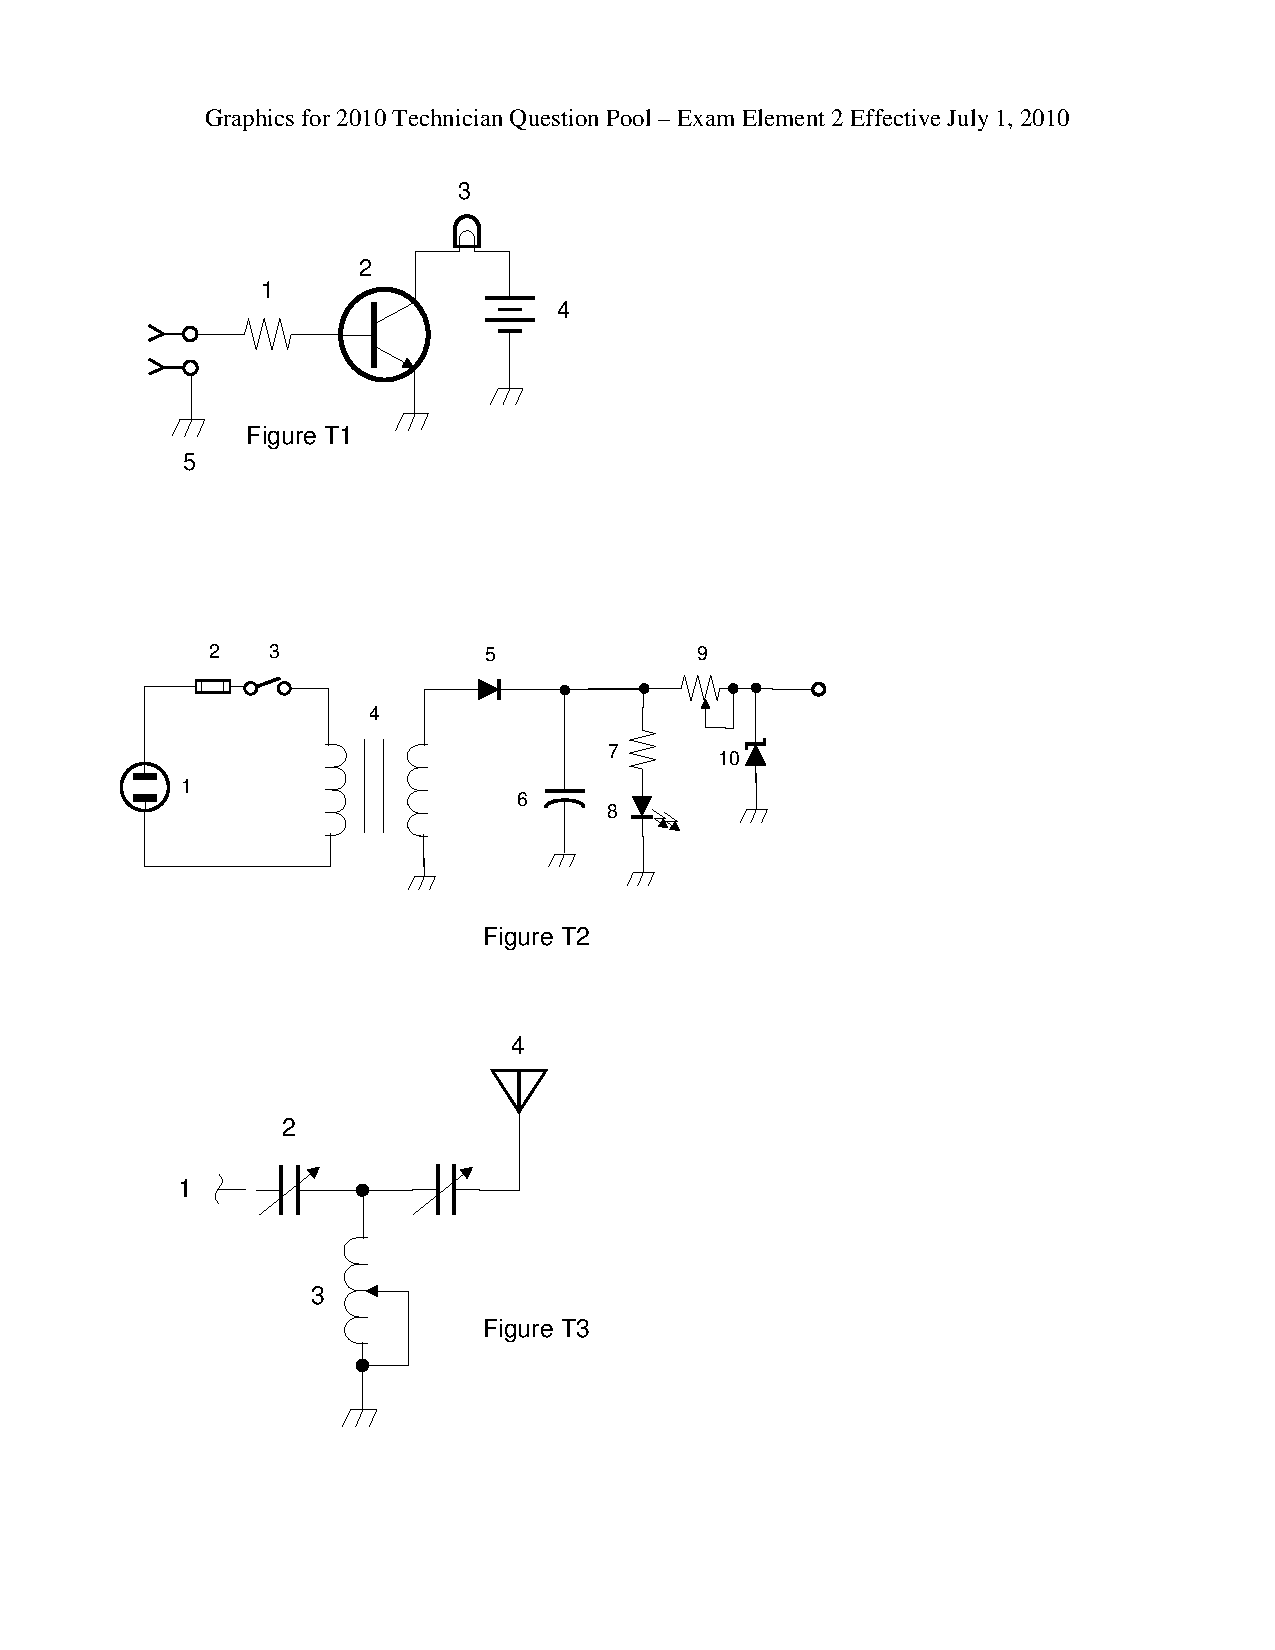
\includepdf[pages={-}]{../sharedfiles/2010element2graphics.pdf}
\end{document}